% !TeX spellcheck = da_DK
\subsection{Referencespænding til Komparator}\label{subsec:Spaendingsref_Komparator}
\subsubsection{Teori og design}
Der skal til komparatorblokken forsynes med en konstant spænding, da denne skal anvendes som sammenligningsgrundlag ift. inputsignalet. Her anvendes igen en referencespænding, som er beskrevet i afsnit \ref{subsec:Spaendingsref} på side \pageref{subsec:Spaendingsref}. Der anvendes samme referencediode til denne referencespænding, som kan ses på \figref{fig:Spaendingsreference}. \\
For at udregne modstanden R1 for referencespændingen til komparatoren benyttes \eqref{eq:udregning_modstand}. Den ønskede referenceværdi er $2.5$V, så der skal i dette tilfælde ikke benyttes en spændingsdeler. I starten af kredsløbet indsættes en operations forstærker (TL$082$), som har to input og output. Derved kan denne fungere som buffer til komparator kredsløbet og den inverterende forstærker. Da spændingen går direkte ind i bufferen, er den maksimale biasstrøm på $50nA$. Biasstrømmen for referencedioden er igen sat til $200\mu$A. Dermed kan værdierne indsættes i formlen og R1 kan beregnes:
\begin{equation}
R_komparator = \frac{5.5V-2.5V}{50nA + 200\mu\text{A} = 14999.62501\Omega \approx 15K\Omega 
\end{equation} 

\subsubsection{Simulering}
Der foretages en simulering i LTspice, for at se hvor præcis spændingsreferencen. TL$082$ fungerer som to TL$081$'ere, og derfor er simuleringen opbygget således:
\begin{figure}[H]
	\centering
	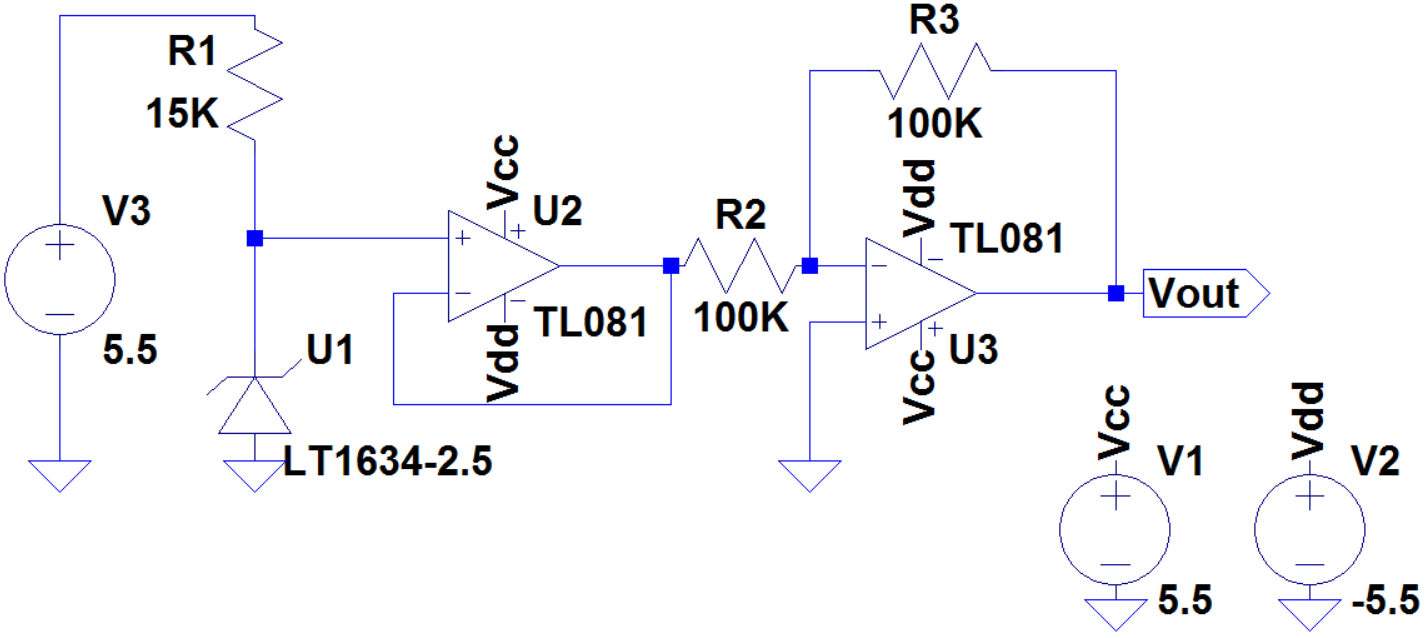
\includegraphics[scale=0.4]{figures/cProblemloesning/Reference_komparator.PNG}
	\caption{På figuren ses designet af referencespændingen til komparatorblokken.}
	\label{fig:ref_komparator}
\end{figure}

Figur af LTspice

 Resultatet af simuleringen kan ses i \tableref{Tab:SpaendingsRef_komparator}

\begin{table}[H]
\centering
\begin{tabular}{|l|l|l|l|}\hline
	& \textit{\begin{tabular}[c]{@{}l@{}}Forventet\\outputsignal\end{tabular}} & \textit{\begin{tabular}[c]{@{}l@{}}Målte\\outputsignal\end{tabular}} & \textit{Afvigelse} \\ \hline
	\textit{\begin{tabular}[c]{@{}l@{}}Input fra\\spændingsforsyning\end{tabular}}      & $...$V             &  $...$V    &   $.\%$         \\ \hline
	\textit{\begin{tabular}[c]{@{}l@{}}Output fra\\spændingsreference\end{tabular}}     & $...$V             &  $...$V    &   $. \%$    \\ \hline
\end{tabular}
\caption{I tabellen ses resultaterne fra simuleringen i LTspice af spændingsreferencen til komparatoren.}
\label{Tab:SpaendigsRef_komparator}
\end{table}


\subsubsection{Implementering og test}